\documentclass{Alexandre}
\usepackage[portuguese, ruled, linesnumbered]{algorithm2e}
\usepackage{multirow}
\usepackage{multicol}
\usepackage{color}
\usepackage{diagbox}
\usepackage{setspace}
\usepackage{listings}
\usepackage{color}
\usepackage{caption}
\usepackage{mwe}
\usepackage[normalem]{ulem}
\usepackage[framemethod=tikz]{mdframed}

\definecolor{codegreen}{rgb}{0,0.6,0}
\definecolor{codegray}{rgb}{0.5,0.5,0.5}
\definecolor{codepurple}{rgb}{0.58,0,0.82}
\definecolor{backcolour}{rgb}{0.95,0.95,0.92}

\lstdefinestyle{mystyle}{
  backgroundcolor=\color{backcolour},   commentstyle=\color{codegreen},
  keywordstyle=\color{magenta},
  numberstyle=\tiny\color{codegray},
  stringstyle=\color{codepurple},
  basicstyle=\footnotesize,
  breakatwhitespace=false,         
  breaklines=true,
  captionpos=b,                   
  keepspaces=true,                 
  numbers=left,                    
  numbersep=5pt,                  
  showspaces=false,                
  showstringspaces=false,
  showtabs=false,                  
  tabsize=2
}

\setbeamertemplate{bibliography item}[triangle]

\title{Ferramenta Colaborativa}
\subtitle{Stack Overflow}
\author{Alexandre Mendonça Fava\inst{1}}


\institute[UDESC]{
  \newline \newline \newline
  \inst{1}
  Mestrado Acadêmico em Computação Aplicada - PPGCA
}

\date{16 Agosto 2019}

\subject{}

\logo{

\includegraphics[scale=0.8]{Figuras/Logo-UDESC.jpg}
}

\begin{document}


\begin{frame}
  \titlepage
\end{frame}
%[Transparência 1] Bom dia, eu me chamo Alexandre, e o sistema utilizado para colaboração que eu escolhi para apresentar foi o Stack Overflow.


\begin{frame}{AGRADECIMENTOS}

    O presente trabalho foi realizado com apoio da Coordenação de Aperfeiçoamento de Pessoal de Nível Superior - Brasil (CAPES) - Código de Financiamento 001. 

\end{frame}
%[Transparência 2] Destaco que o presente trabalho sobre o Stack Overflow foi realizado com total apoio da CAPES.


\begin{frame}{APRESENTAÇÃO}

    \begin{figure}
        
\includegraphics[scale = 0.2]{Figuras/Logo-StackOverflow.png}
    \end{figure}

\end{frame}
%[Transparência 3] Antes de começar, eu gostaria de saber: quem aqui conhece o Stack Overflow?


\begin{frame}{CRIADORES}

    \begin{figure}
        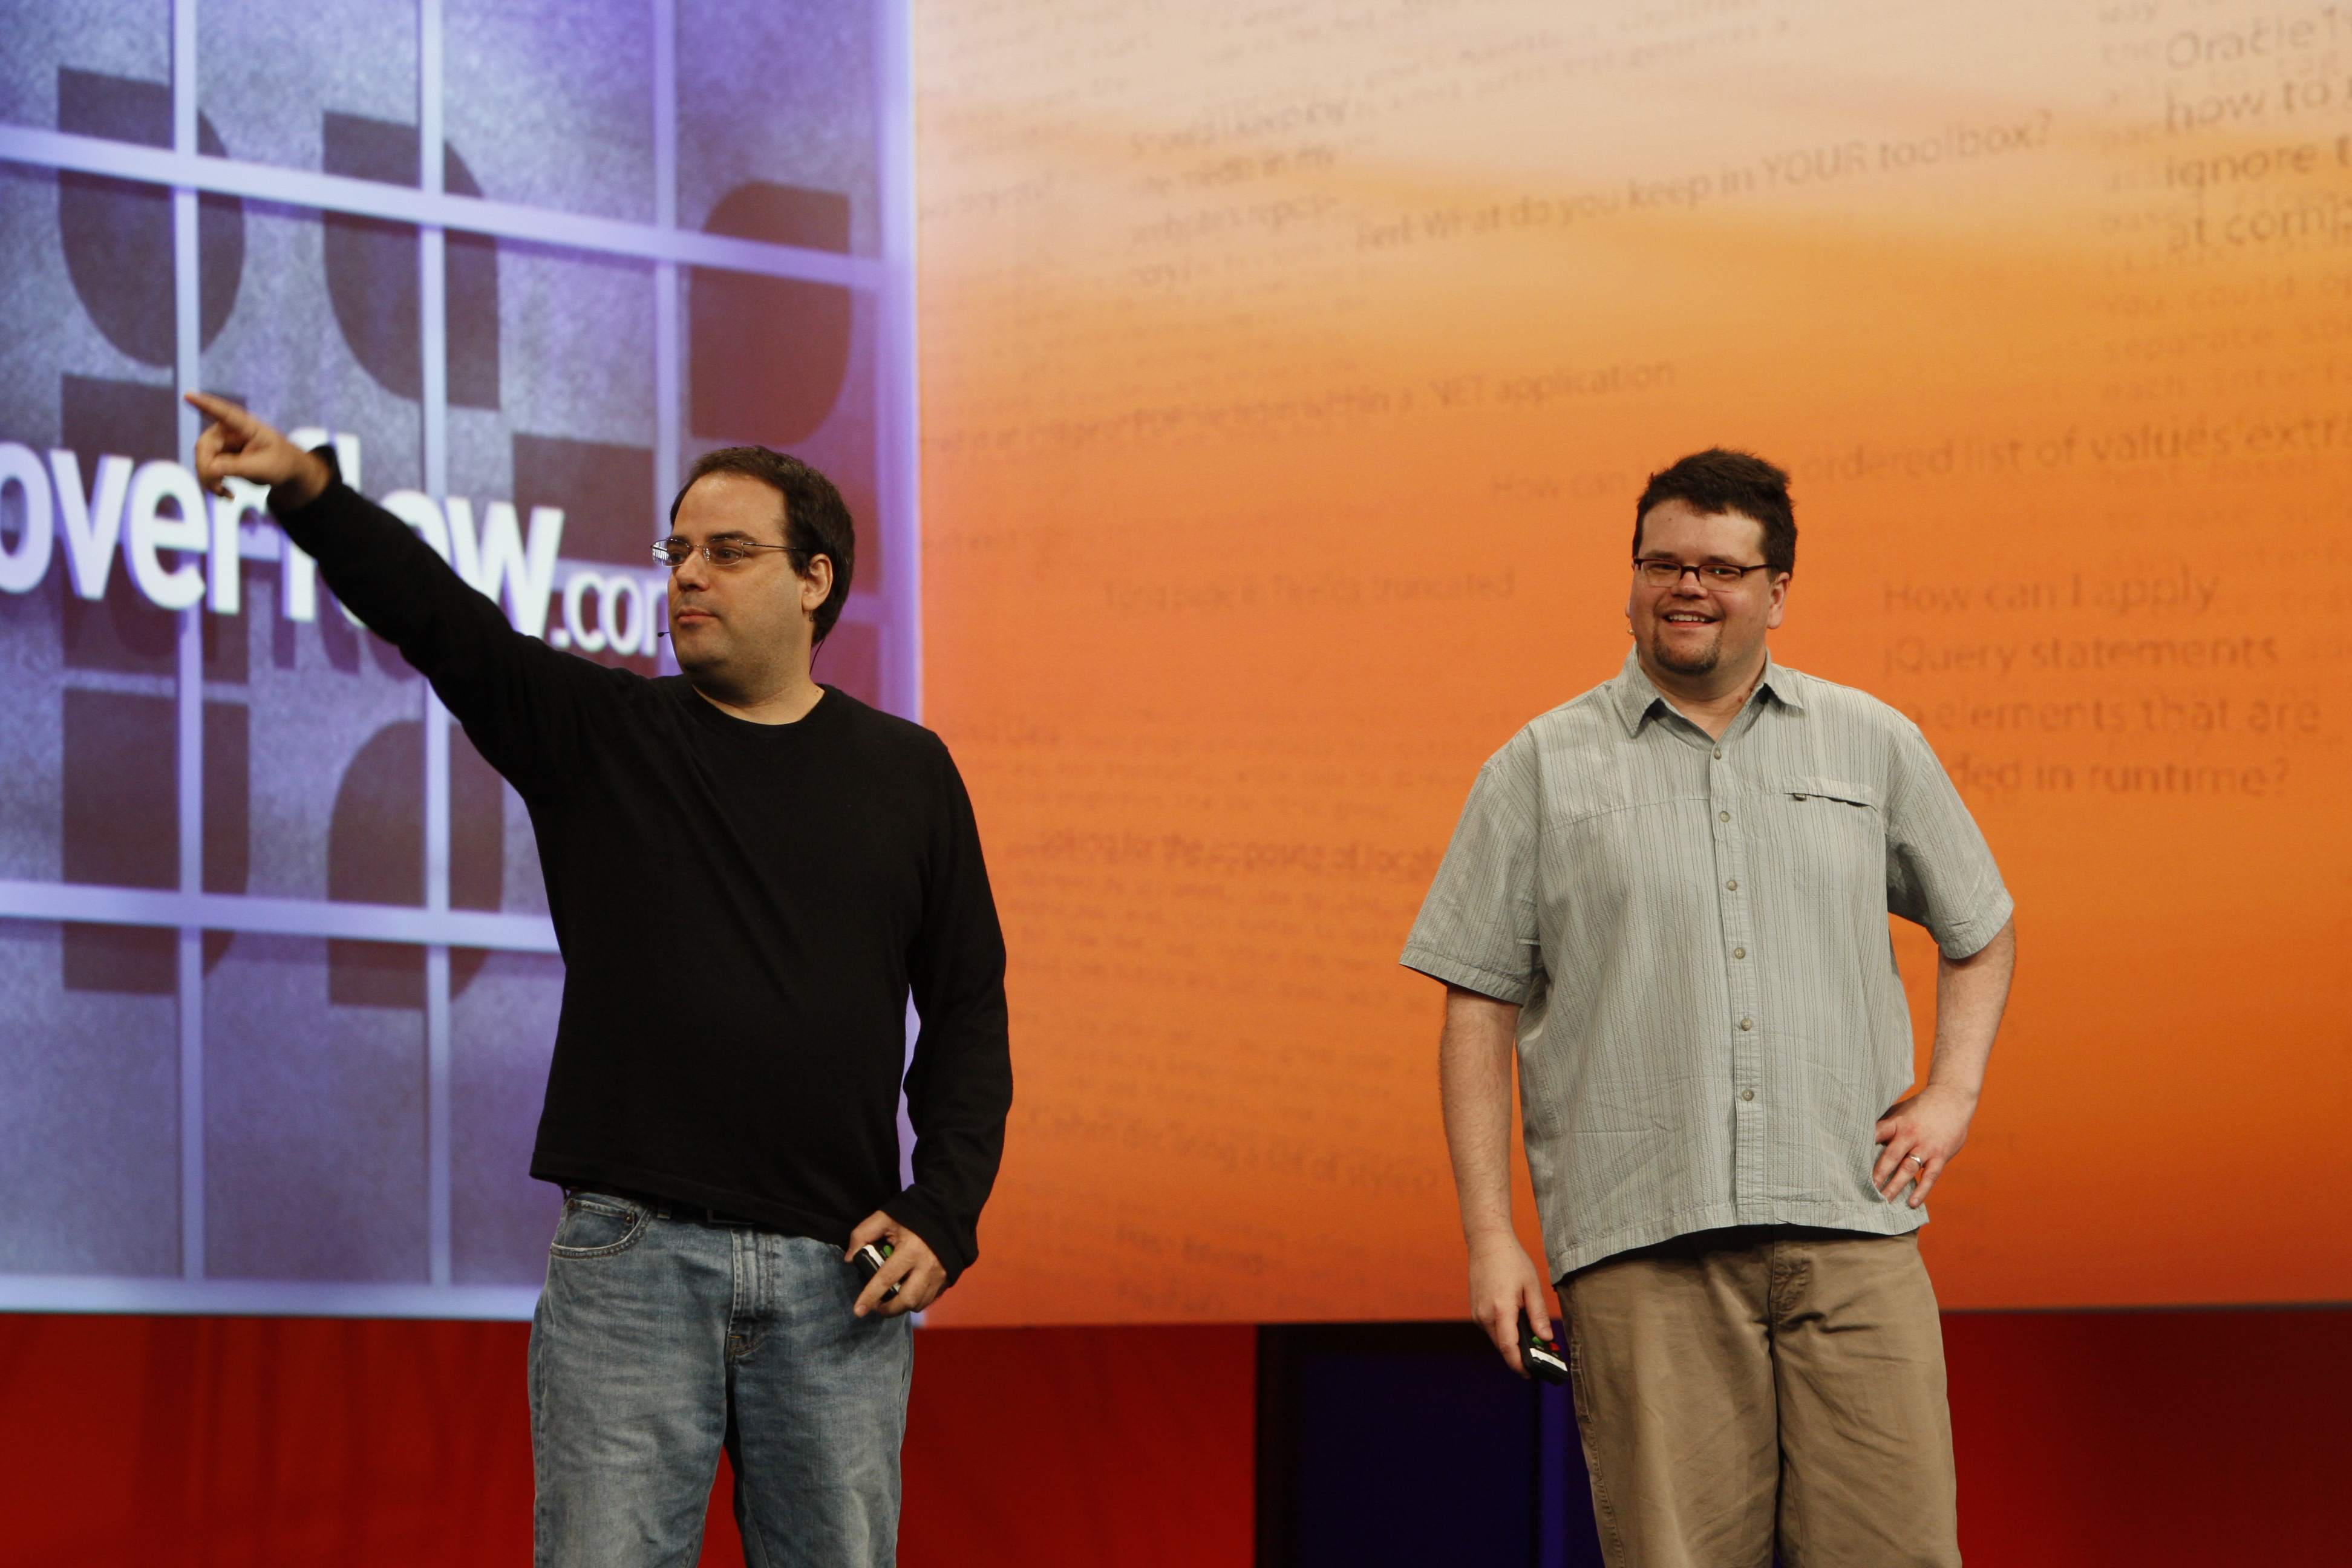
\includegraphics[scale = 0.06]{Figuras/Criadores-StackOverflow.jpg}
    \end{figure}

\end{frame}
%[Transparência 4] O Stack Overflow foi idealizado e desenvolvido por um programador e por um Engenheiro de Software: Joel Spolsky[esquerda] e Jeff Atwood[direita].


\begin{frame}{CRIATURAS}

    \begin{figure}
        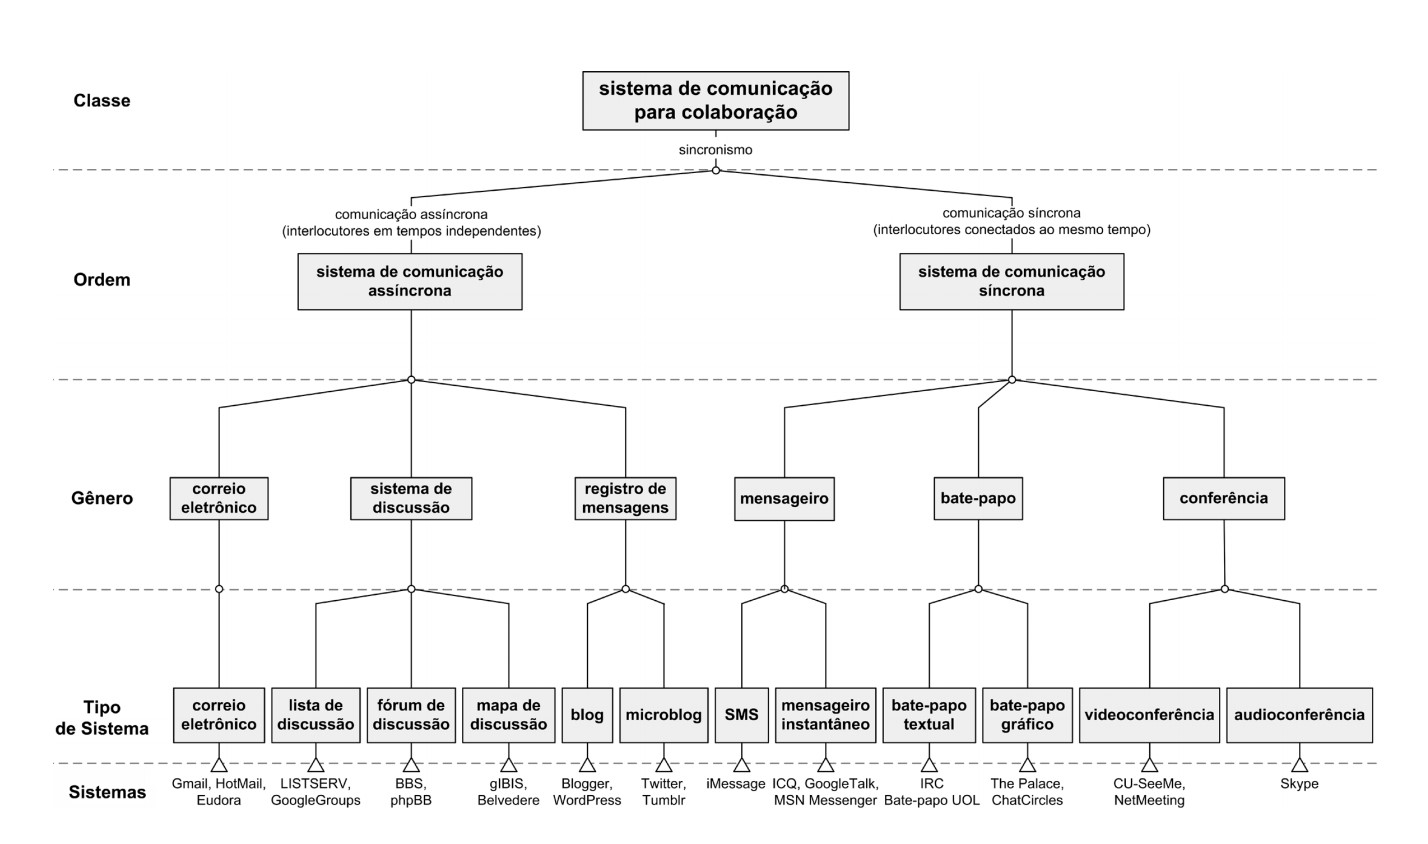
\includegraphics[scale = 0.27]{Figuras/FerrametasColaborativas.jpg}
    \end{figure}

\end{frame}
%[Transparência 5] E o que de fato eles criaram? Sabemos que é uma ferramenta colaborativa, mas que tipo de ferramenta colaborativa?
%O Stack Overflow se encontram obviamente na CLASSE de 'sistema de comunicação para colaboração'
%Mais especificamente, a sua ORDEM é de um 'sistema de comunicação assíncrona'
%O seu GÊNERO é de um 'sistema de discussão'
%E por fim, o seu TIPO é um 'fórum de discussão'


\begin{frame}{OBJETIVO}

    \begin{figure}
        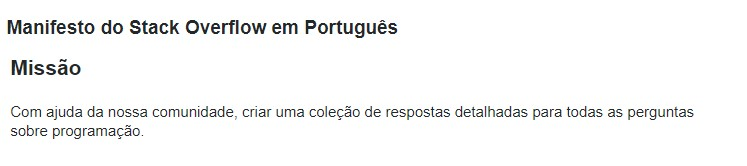
\includegraphics[scale = 0.6]{Figuras/Manifesto-StackOverflow.jpg}
    \end{figure}

\end{frame}
%[Transparência 6] Ok, já sabemos que é um fórum de discussão, para qual tipo de discussão? 
%Qual é o objetivo desse fórum? 
%Para descobrir isso, basta ler o manifesto no site oficial do Stack Overflow


\begin{frame}{FUNCIONAMENTO}

    \begin{figure}
        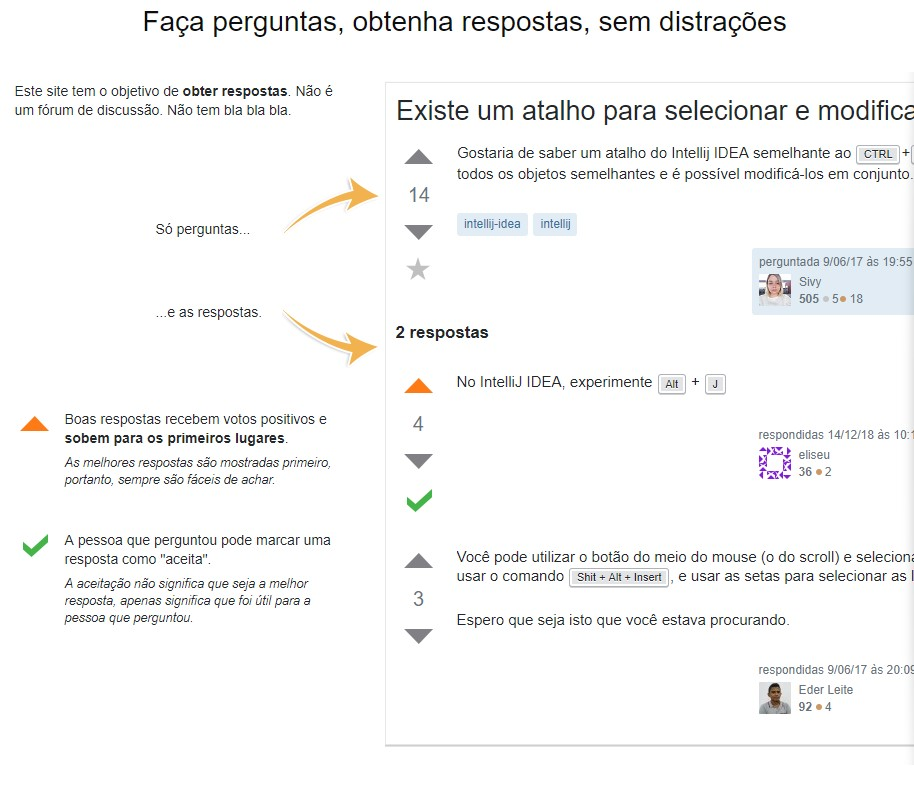
\includegraphics[scale = 0.35]{Figuras/StackOverflow-Perguntas.jpg}
    \end{figure}

\end{frame}
%[Transparência 7] Ou seja, seu funcionamento se dá através de preguntas e respostas sem distrações.
%E embora o tipo dele seja um FÓRUM DE DISCUSSÃO. Suas diretrizes dizem que não é um fórum de discussão. Pois o objetivo não é discutir, é feita uma pergunta e é dada uma resposta, PONTO. Sem discussão.


\begin{frame}{FUNCIONAMENTO}

    \begin{figure}
        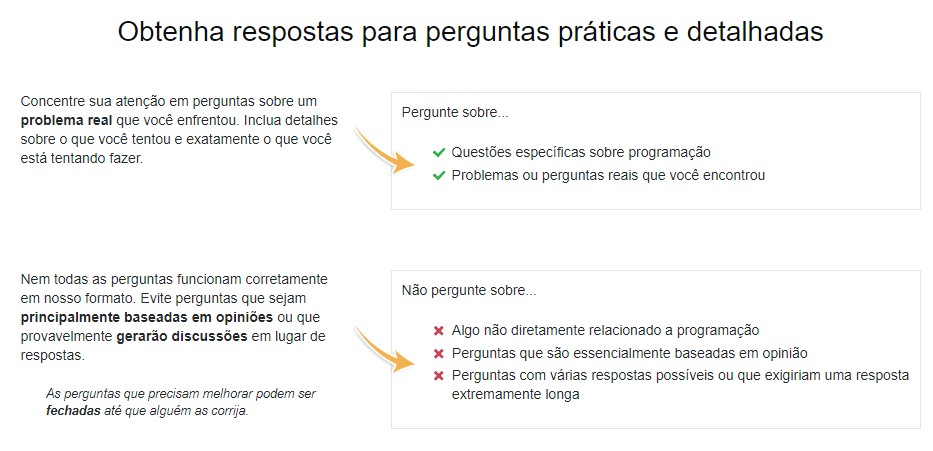
\includegraphics[scale = 0.4]{Figuras/StackOverflow-Respostas.jpg}
    \end{figure}

\end{frame}
%[Transparência 8] Nada que possa GERAR DISCUSSÕES é aceito. Onde perguntas do tipo pode ser fechadas.


\begin{frame}{FUNCIONAMENTO}

    \begin{figure}
        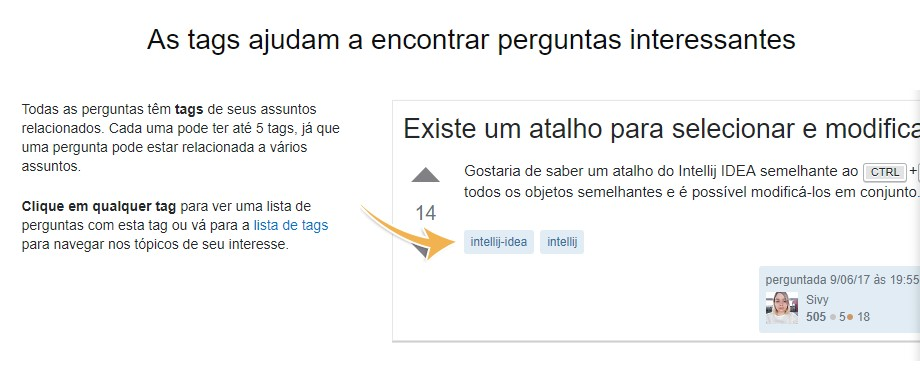
\includegraphics[scale = 0.45]{Figuras/StackOverflow-Etiquetas.jpg}
    \end{figure}

\end{frame}
%[Transparência 9] No caso das perguntas, é de suma importância incluir TAGS ou ETIQUETAS nas perguntas, para assim o sistema estruturar melhor todo o conteúdo gerado. Todas a perguntas devem ter etiquetas, pois toda a pergunta está relacionada a algum assunto, pelo menos: seja linguagem de programação, ou outra coisa.


\begin{frame}{FUNCIONAMENTO}

    \begin{figure}
        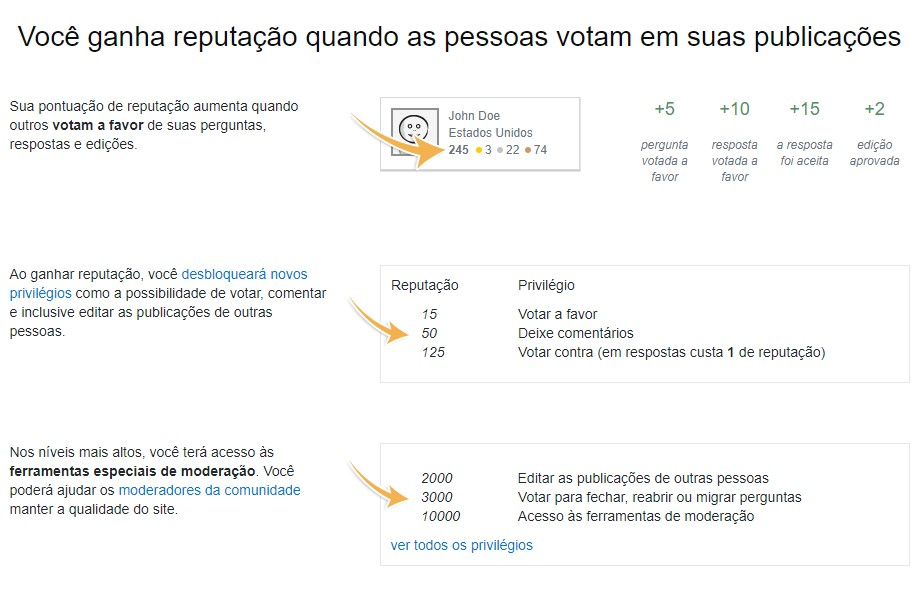
\includegraphics[scale = 0.35]{Figuras/StackOverflow-Recompensa.jpg}
    \end{figure}

\end{frame}
%[Transparência 10] O Stack Overflow trabalha com uma espécie de sistema de gamificação (ludificação), encorajando assim seus usuários a fazerem perguntas e a responderem perguntas. 


\begin{frame}{FUNCIONAMENTO}

    \begin{figure}
        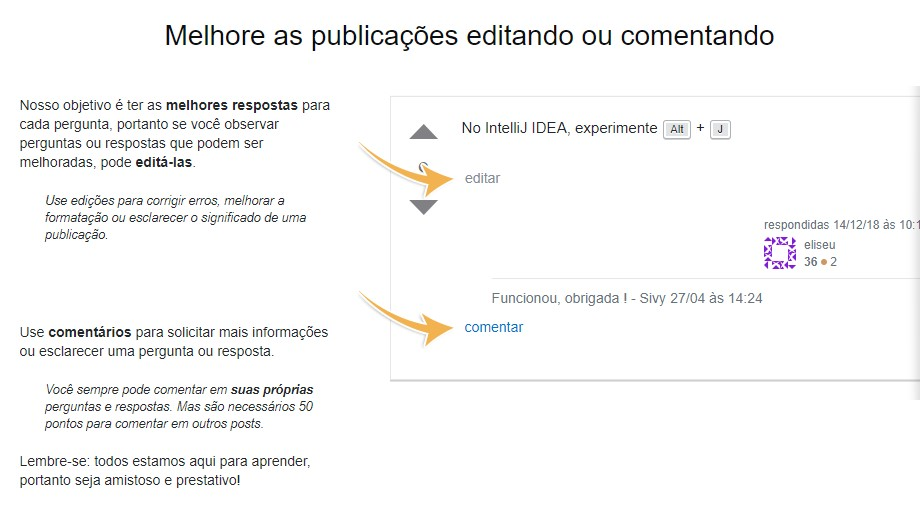
\includegraphics[scale = 0.4]{Figuras/StackOverflow-Edicao.jpg}
    \end{figure}

\end{frame}
%[Transparência 11] O Stack Overflow também trabalha com edições e comentários. Com as edições ajudando a polir uma determinada pergunta ou resposta. E com os comentários ajudando a esclarer outros usuários o quanto aquela resposta ajudou.


\begin{frame}{FUNCIONAMENTO}

    \begin{figure}
        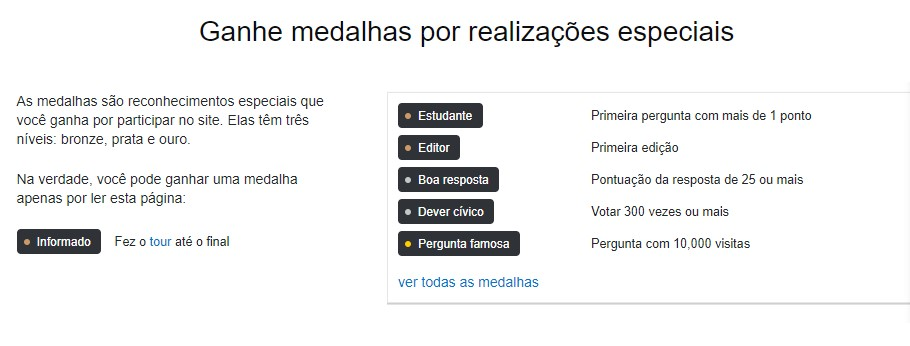
\includegraphics[scale = 0.45]{Figuras/StackOverflow-Recompensas.jpg}
    \end{figure}

\end{frame}
%[Transparência 12] Por fim, o Stack Overflow trabalha também com recompensas, fornecendo medalhas aos usuários quando determinadas conquistas são alcançadas, se assemlhando mais ainda com a ideia de gamificação (ludificação).


\begin{frame}{OUTRAS FERRAMENTAS}

    \begin{figure}
        
\includegraphics[scale = 0.65]{Figuras/YahooRespostas.jpg}
    \end{figure}

\end{frame}
%[Transparência 13] Depois dessa breve introdução sobre o Stack Overflow, a pergunta que fica é: 
%Mas qual a diferença dele para o Yahoo Respostas, por exemplo?
%Por ser voltada a programação, o Stack Overflow disponibiliza ferramentas de 'coloração de sintaxe' (Syntax highlighting)
%Além disse o Stack Overflow FECHA as perguntas que tiveram avaliação ruins, diferente do Yahoo.
%Mas a verdade é que o Stack Overflow não é especial 


\begin{frame}{OUTRAS FERRAMENTAS}

    \begin{figure}
        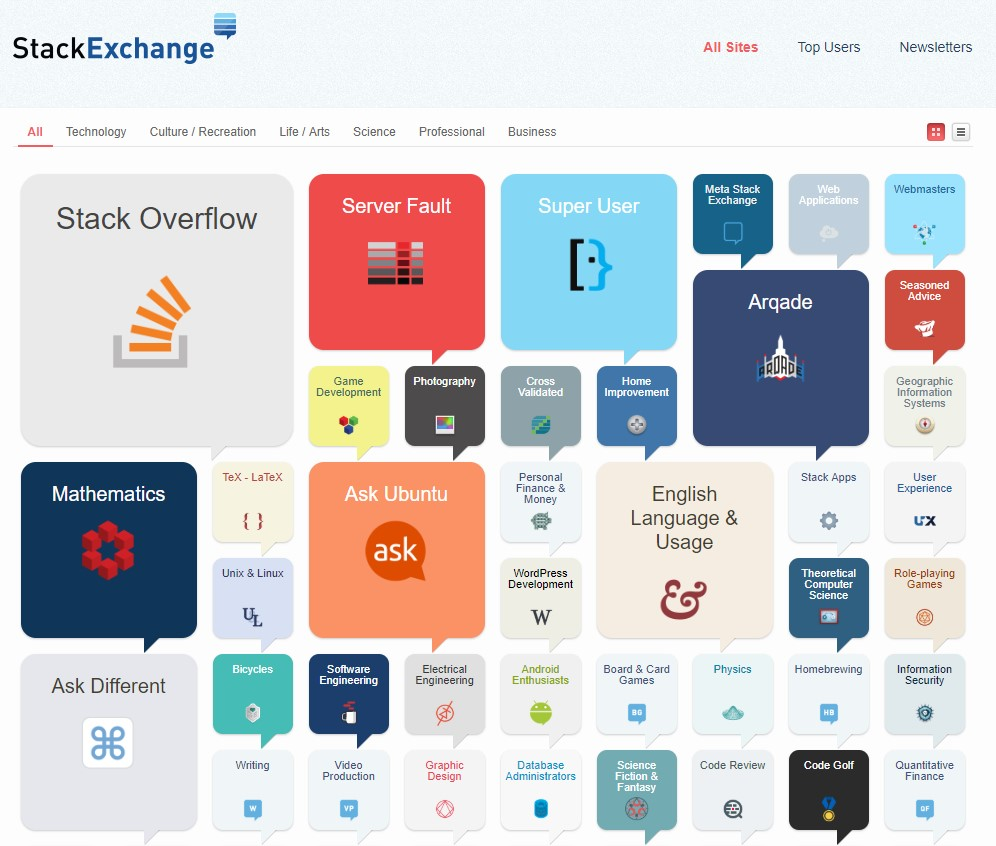
\includegraphics[scale = 0.35]{Figuras/Outros.jpg}
    \end{figure}

\end{frame}
%[Transparência 14] O Stack Overflow na verdade, é apenas uma parte de uma rede de mais de 170 sites de perguntas e respostas, intitulada de Stack Exchange.


\begin{frame}{NÚMEROS}

    \begin{figure}
        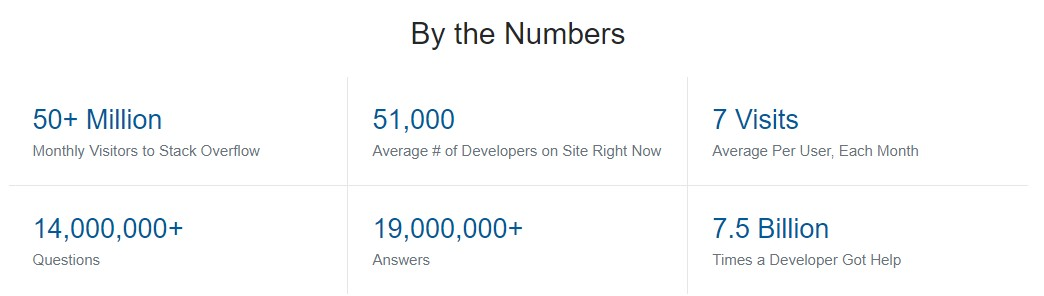
\includegraphics[scale = 0.35]{Figuras/Numeros.jpg}
    \end{figure}
    
    \textbf{Ranking: }
    \begin{itemize}
        \item  46º [Brasil]   
        \item  43º [Mundo]
    \end{itemize}

\end{frame}
%[Transparência 15] Tudo bem que o Stack Overflow é o de maior destaque desta rede, com números gigantescos. Mas perto de outros gigantes, o Stack Overflow é bastante modesto.


\begin{frame}
    \begin{center}
        \begin{figure}{\textit{"I Learned to Stop Worrying And Love Duplication"}}
            
\includegraphics[scale = 0.45]{Figuras/Jeff.png}
            \textit{ - Jeff Atwood, 2010}
        \end{figure}
    \vspace{1.5cm}

    \begin{Huge} 
    Obrigado!\\
    \end{Huge}
    \bigskip
    Alexandre Mendonça Fava - \alert{alexandre.fava@hotmail.com}\\
    \end{center}
\end{frame}

\end{document}